% Text-pass fixture: links (hyperref), cross-references, a French passage and coloured
% text (xcolor). Written for ReadableSTEM's tests; no third-party text. Build: make_pdfs.py.
\documentclass[11pt]{article}
\usepackage[T1]{fontenc}
\usepackage{lmodern}
\usepackage{amsmath}
\usepackage{xcolor}
\usepackage{tikz}
\usepackage[margin=1in]{geometry}
% Links keep the body colour (no boxes, no coloured link text): colour in this fixture
% comes only from \textcolor, so the colour tests and the link tests stay apart.
\usepackage[hidelinks]{hyperref}
\usepackage{xurl}
\pagestyle{empty}

\begin{document}

\section{Course links}

The \href{https://example.org/physics/syllabus}{course syllabus} lists the reading for
every week, and questions go to
\href{mailto:instructor@example.edu}{the instructor by email}. Last year's notes are at
\url{https://example.org/physics/archive/2025/lecture-notes/week-01-kinematics.pdf} and
the problem sets are \href{https://example.org/physics/problems}{here}. The lab data is
on an old \href{ftp://ftp.example.org/lab/data.csv}{file server} that the PDF still
links to.

\section{Motion with constant acceleration}

A cart that starts with speed $v_0$ and speeds up at a steady rate $a$ has, after a time
$t$, the speed
\begin{equation}
  v = v_0 + a t
  \label{eq:speed}
\end{equation}
and has covered the distance
\begin{equation}
  x = v_0 t + \tfrac{1}{2} a t^2 .
  \label{eq:distance}
\end{equation}
Eliminating $t$ between Eqs.~(\ref*{eq:speed}) and~(\ref*{eq:distance}) gives the third
relation of the section. Equation~\eqref{eq:speed} holds for any steady rate, and so does
Eq.~\ref*{eq:distance}; Figure~\ref*{fig:cart} shows the cart, and
Figure~\ref{fig:cart} links to it from the PDF itself.

\begin{figure}[h]
  \centering
  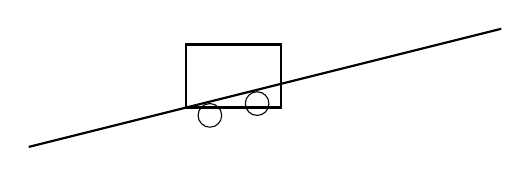
\begin{tikzpicture}
    \draw[thick] (0,0) -- (6,1.5);
    \draw[thick] (2,0.5) rectangle (3.2,1.3);
    \draw (2.3,0.4) circle (0.15);
    \draw (2.9,0.55) circle (0.15);
  \end{tikzpicture}
  \caption{A cart on a ramp.}
  \label{fig:cart}
\end{figure}

\section{A note in French}

The exam has one question written in French, quoted here as it will be printed:
\begin{quote}
La vitesse moyenne est le quotient du d\'eplacement par la dur\'ee du trajet, et elle
s'exprime en m\`etres par seconde.
\end{quote}

\section{Colour in the notes}

In these notes, \textcolor{red}{the vectors are printed in red} and scalars in black, so
read the terms shown in red as vectors. \textcolor{gray!35}{A light grey hint follows
each problem.} \textcolor{black!85}{This sentence is dark grey, which reads as black.}

\end{document}
